\cleardoublepage
\section{MTU Bestimmung}
\label{sec:MTU Bestommung}

Um die bei der Analyse erwähnten Probleme von \acs{PMTUD} zu vermeiden wird die \acs{MTU} vom \tool{} innerhalb des \acs{VPN} Tunnels festgestellt.

Dazu werden \acs{ICMP} Pakete vom Typ \enquote{ICMPv4TypeEchoRequest} und \enquote{ICMPv4TypeEcho-Reply} verwendet. Diese Pakete werden wie bei \acs{PMTUD} mit einem \enquote{Don't fragment} Flag versehen. Im Unterschied zu \acs{PMTUD} werden sie aber im \acs{VPN} Tunnels übermittelt und werden daher in \acs{ESP}s gekapselt. Ausserhalb des Tunnels sind die ICMP Pakete des \tool{}s so nicht unterscheidbar vom normalen Verkehrs und können nicht blockiert werden.
Der \enquote{Don't fragment} Flag jedoch wird bis in die \acs{ESP} Hülle weitergezogen so dass auch das \acs{ESP} welches das \acs{ICMP} Paket transportiert nicht fragmentiert wird.

\begin{figure}[H]
    \begin{center}
        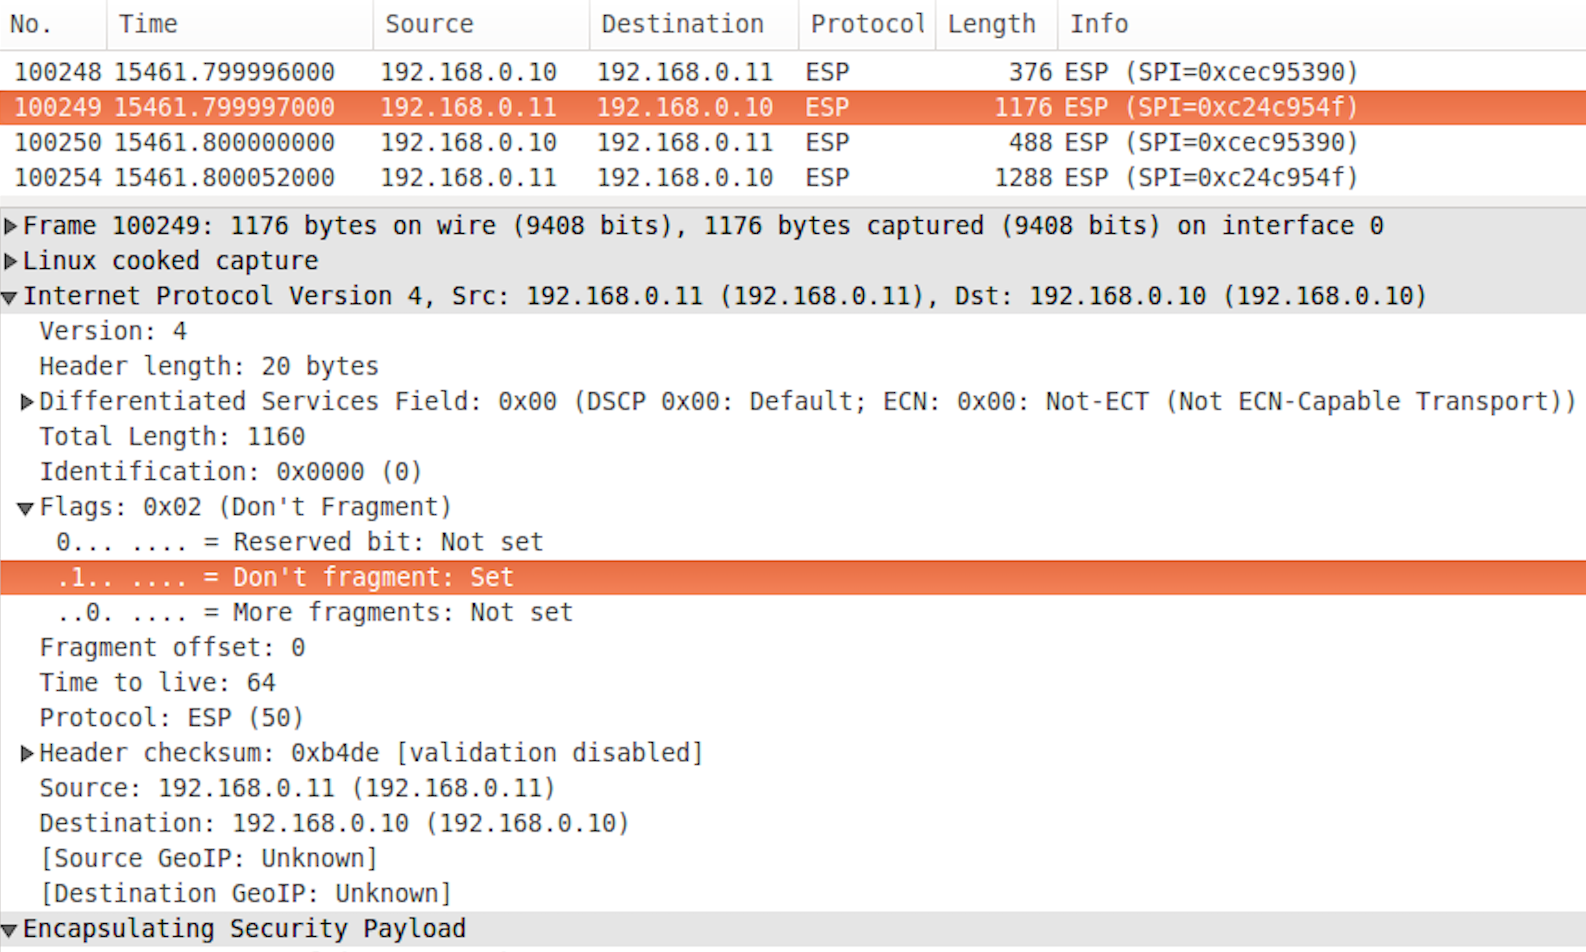
\includegraphics[trim=1 0 0 0,clip,width=\textwidth]{mainpart/implementation/img/ESP_DontFragment}
    \end{center}
    \caption{In ESP gekapseltes ICMP Paket mit \enquote{Don't fragment} flag.}
\end{figure}

Um den \acs{MTU} Discovery Vorgang zu starten wird jeweils ein \enquote{ICMPv4TypeEchoRequest} versendet. Wenn der Ziel Computer das Paket erhält dann sendet er ein Ping Reply mit dem gleichen Paketinhalt zurück.

\begin{figure}[H]
    \begin{center}
    		% GFX Trim left bottom right top
        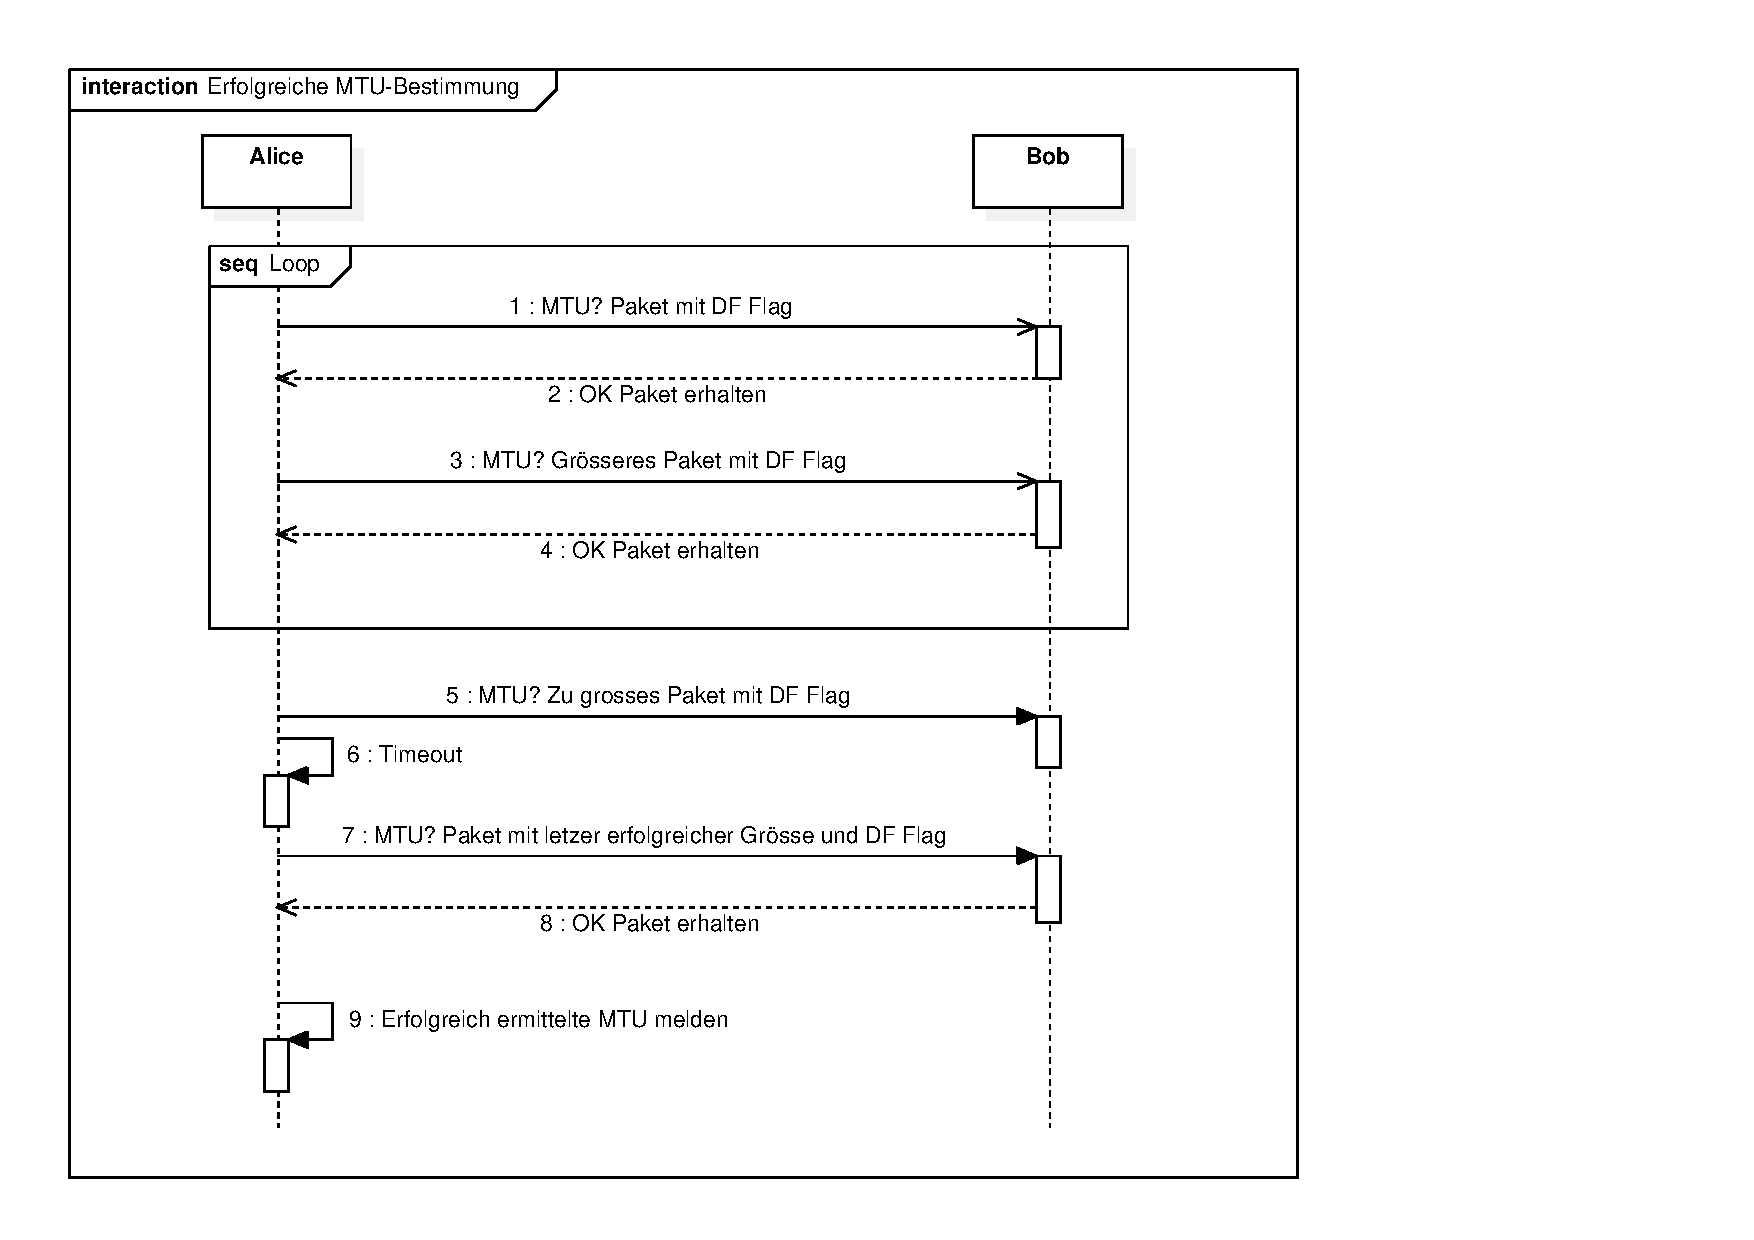
\includegraphics[trim=30 80 140 20,clip,width=\textwidth]{mainpart/implementation/img/MTUBestimmungErfolgreich}
    \end{center}
    \caption{Vereinfachter Ablauf der MTU Bestimmung}
\end{figure}

Die obenstehende Grafik zeigt den weiteren Ablauf der \acs{MTU} Bestimmung mit dem \tool{}. Alice sendet ein \enquote{ICMPv4TypeEchoRequest} Paket und einer bestimmten Grösse an Bob. Wenn Bob das Paket erhält, sendet er ein \enquote{ICMPv4TypeEchoReply} Paket mit derselben Grösse als Antwort. Alice erhöht darauf die Paketgrösse und schickt erneut ein \enquote{ICMPv4TypeEchoRequest} an Bob. Dies wird so lange wiederholt bis das Paket nicht mehr ankommt. Bob erhält also das \enquote{ICMPv4TypeEchoRequest} Paket nicht und kann somit Alice auch keine Antwort schicken. Alice wartet nun einen konfigurierten Timeout ab. Wenn innerhalb des Timeouts keine Antwort ankommt geht Alice davon aus dass das Paket aufgrund der \ac{MTU} von Bob verloren gegangen ist. So lässt sich die \ac{MTU} zwischen Alice und Bob ermitteln.

\subsection{MTU-Discovery Algorithmus - Erster Prototyp}
Für den ersten Prototyp des \tool{} haben wir die \ac{MTU} Discovery auch wie oben beschrieben implementiert. Es wurden also immer ein Request abgeschickt und dann auf eine Antwort gewartet. Die Idee dabei war die \ac{MTU} mithilfe des Binary Search Algorithmus zu finden. 

\begin{lstlisting}[language=bash, caption=MTU Discovery in Binary Search]                    
Range 0		-	2000 --> Trying 1000
Range 1000	-	2000 --> Trying 1500
Range 1500	-	2000 --> Trying 1750
Range 1500	-	1750 --> Trying 1625
Range 1500	-	1625 --> Trying 1562
Range 1500 	-	1563 --> Trying 1532
Range 1500	-	1532 --> Trying 1516
Range 1500	-	1508 --> Trying 1504
Range 1500	- 	1504 --> Trying 1502
Range 1500	-	1502 --> Trying 1501
Range 1500 	- 	1501 --> Exact MTU detected
\end{lstlisting}

Wie man der Darstellung (oben) erkennen kann braucht man 11 Versuche um die exakte \ac{MTU} in einem Range von 0-2000 Bytes zu finden. So lange die Antwortszeit zwischen Alice und Bob klein ist funktioniert diese Art der \ac{MTU} Bestimmung somit gut und zuverlässig.

Beim Mitte-Projekt Meeting mit dem Industriepartner kam dann aber die Frage auf was passiert wenn man die \ac{MTU} auf einer sehr langsamen Verbindung feststellen möchte. So betreibt die \osag einige Verbindungen die noch via Satelliten-Link angebunden sind. Bei solchen Verbindungen sind gemäss der \osag Timeouts von 10 Sekunden realistisch. Wenn jetzt also beim Binary Search Algorithmus für jedes Paket das nicht ankommt auf ein 10 Sekunden Timeout gewartet werden muss dann dauert die \ac{MTU} Discovery ganz schön lange. Und so haben wir uns nochmals Gedanken gemacht wie man die \ac{MTU} mit einem ähnlichen Algorithmus, aber in wenigen Schritten finden kann.

\subsection{MTU-Discovery Algorithmus - FastMTU}
FastMTU war die Lösung unserers Problems 














\todo{REMOVE:}
Bei FastMTU bleibt das grundlegende Prinzip der \acs{MTU} Bestimmung gleich, es werden Pakete unterschiedlicher Grösse versendet so dass man herausfinden kann welche ankommen und welche verworfen werden. Neu wird jedoch nicht nur ein Paket aufs Mal versendet sondert einen ganze Batch von Paketen. Dazu wird aus der Konfiguration einen sogenannter Range ausgelesen. Der Range besteht aus zwei Byte-Grössen die festlegen worin sich die \acs{MTU} typischerweise befinden sollte. Zum Beispiel zwischen 0 und 2000 Bytes. Dann wird aus der Konfiguration ausgelesen wie viele Pakete aufs Mal versendet werden sollen. Mehr gleichzeitige Pakete führen zu einer schnelleren Bestimmung der \acs{MTU}, haben aber auch zur Folge dass die \acs{VPN} Verbindung stärker belastet wird und so möglicherweise wichtiger Kunden-Traffic ausgebremst wird. Als Default-Wert gehen wir von 20 gleichzeitigen Paketen aus. Der Range 0-2000 Bytes wird jetzt also durch 20 geteilt. Damit erhält man 20 Pakete die sich je um 100 Bytes unterscheiden. Diese 20 Pakete werden nun als einen Batch versendet.
Für alle Pakete die auf der anderen Seite des Tunnels ankommen wird nun eine Antwort generiert. Bei einer MTU von 1500 Bytes würden die ersten 15 Pakete ankommen. Der Sender weiss jetzt also dass die exakte \acs{MTU} zwischen dem letzten erfolgreichen Paket (1500) und dem ersten nicht erfolgreichen Paket (1600) sein muss. 1500-1600 Bytes wird nun als neuer Range gesetzt und erneut durch die Anzahl gleichzeitiger Pakete geteilt. Die Pakete des zweiten Batches haben jetzt noch 5 Bytes Unterschied. Dieser Vorgang wird so lange wiederholt bis der Unterschied zwischen den Paketen eines Batches nur noch 1 Byte sind. Dadurch weiss der Algorithmus wenn die exakte \acs{MTU} gefunden wurde.

Bei einer MTU zwischen 0-2000 Bytes werden 3 Batches an Paketen versendet. Pro Batch muss jeweils die Dauer des Timeout-Timers gewartet werden. Daher lässt sich bereits im voraus sagen wie lange das Finden der exakten \acs{MTU} mit FastMTU dauern wird. Gerade in Gegenden die noch per Satelliten-Link angebunden sind kann es durchaus mal länger bis alle Pakete ankommen. Gemäss der \osag ist ein Timeout von 10 Sekunden für solche Verbindungen realistisch. Das Bestimmen der \acs{MTU} zwischen 0 und 2000 Bytes hätte also 30 Sekunden gedauert.
Die verbrauchte Zeit beim Bestimmen von FastMTU lässt sich sehr leicht via der Konfiguration optimieren. So hat man die Möglichkeit den Range stärker einzuschränken, den Timeout zu verkürzen oder aber mehr Pakete pro Batch zu versenden.

\begin{figure}[H]
    \begin{center}
        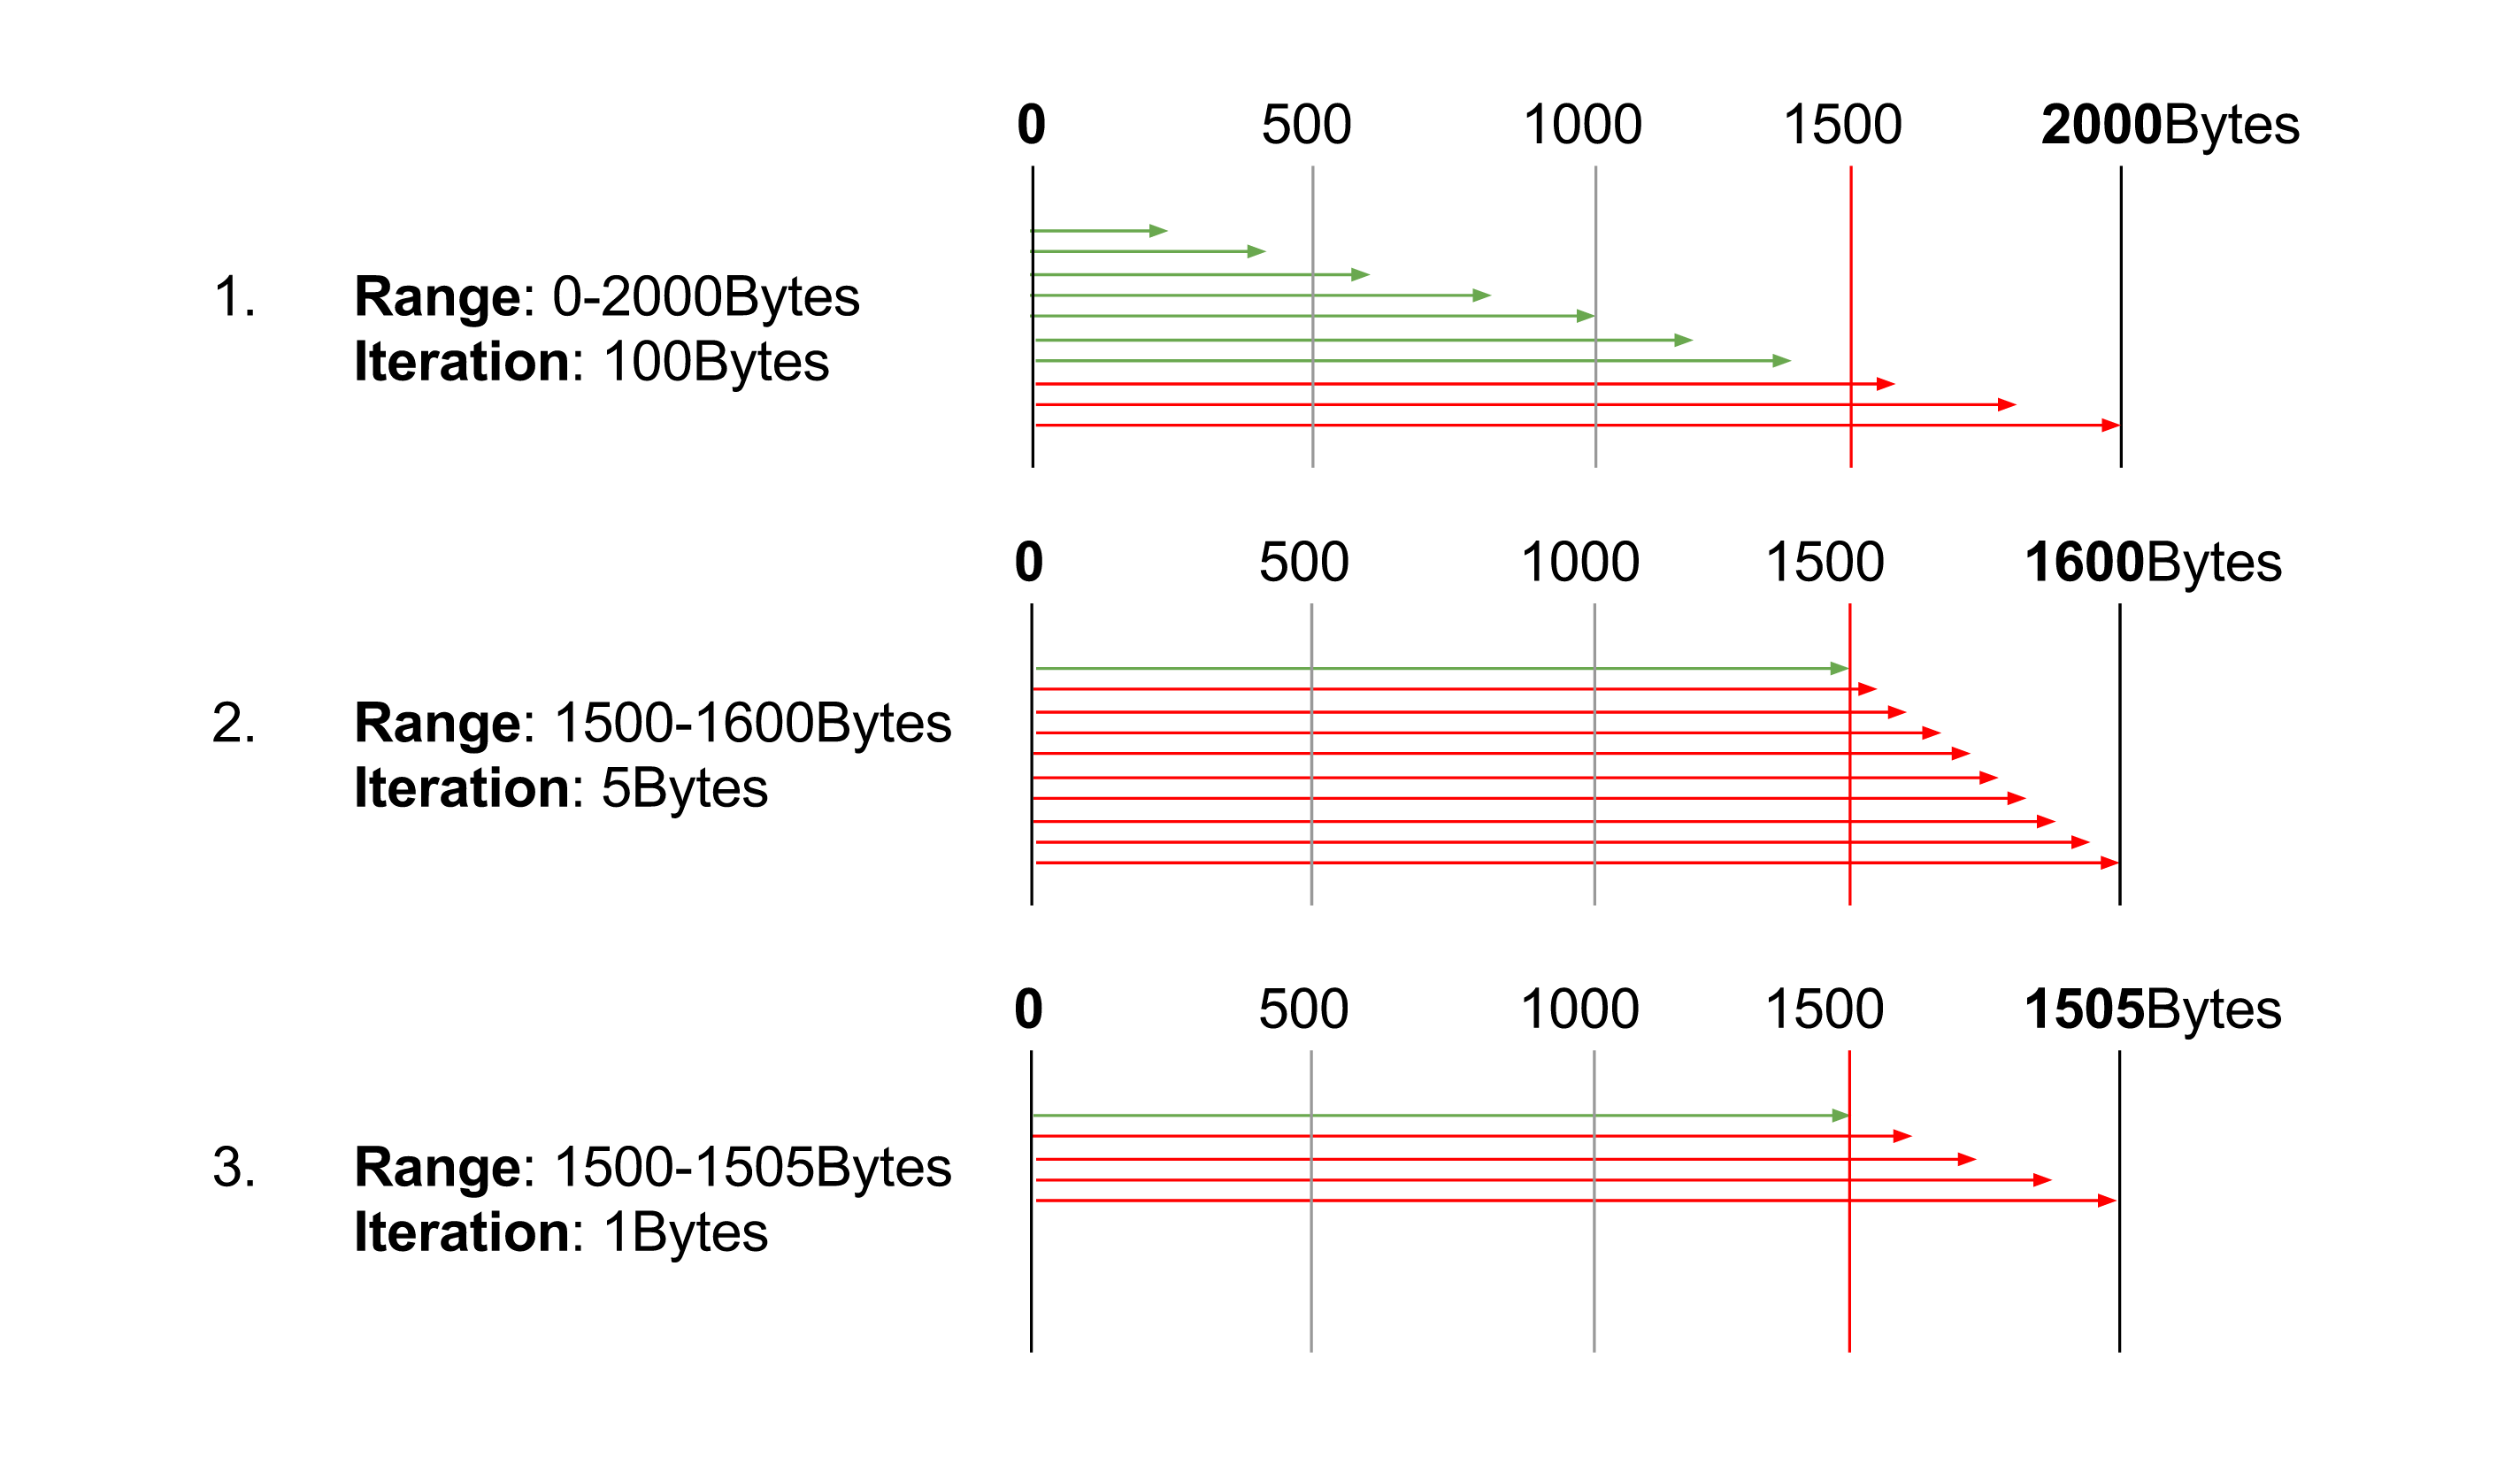
\includegraphics[clip,width=\textwidth]{mainpart/implementation/img/FastMTUAlgorithm}
    \end{center}
    \caption{Ablauf einer MTU Discovery zwischen 0 und 2000Bytes}
\end{figure}

Auch wenn die \acs{MTU} sich ausserhalb des Ranges befindet wird sie von FastMTU noch korrekt detektiert. Wenn nämlich alle Pakete eines Batches eine erfolgreiche Antwort der Gegenseite generieren, dann wird der nächste Range einfach um die Grösse des überprüften Range vergrössert. Im Beispiel mit einem Range von 0-2000 Bytes würde jetzt einfach 2000-4000 Bytes überprüft.